% CNET Phase IV paper. Build: pdflatex main && bibtex main && pdflatex main && pdflatex main
% RULE: every number in this file comes from a committed result record named in a comment next
% to it. \pending{...} marks a value that is not yet verified; the PDF must contain none at submission.
\documentclass[journal]{IEEEtran}
\usepackage[T1]{fontenc}
\usepackage{amsmath,amssymb}
\usepackage{booktabs,multirow,array}
\usepackage{graphicx}
\usepackage{xcolor}
\usepackage{tikz}
\usetikzlibrary{arrows.meta,positioning,fit,backgrounds}
\usepackage{algorithm}
\usepackage{algpseudocode}
\usepackage[hidelinks]{hyperref}
\usepackage{cite}

\newcommand{\pending}[1]{\textcolor{red}{\textbf{[PENDING: #1]}}}
\newcommand{\dd}{\mathrm{d}}

\begin{document}

% ===================================================================== 1. Title and authors
\title{How Real Is 99\% Accuracy? Auditing Feature Reliance in Network Intrusion Detection}
\author{\pending{Author names, roll numbers and affiliation (FAST-NUCES Islamabad)}%
\thanks{Course project, Computer Networks (CNET), FAST-NUCES, 2026.}}
\maketitle

% ===================================================================== 2. Abstract
\begin{abstract}
\pending{150--250 words, written last from verified numbers only: (i) problem: near-perfect NIDS
scores on CICIDS2017; (ii) method: duplicate-aware split, model-visible twin exclusion,
literature-defined artifact groups with size-matched random controls, 10 paired seeds, exact
sign-flip tests with Holm correction and TOST equivalence, untouched Monday benign FPR, and
transfer to the Engelen corrected capture; (iii) AE-XGBoost results; (iv) DCNN official vs
duplicate-filtered results; (v) MES-DNN random vs duplicate-aware results; (vi) conclusion.}
\end{abstract}

% ===================================================================== 3. Keywords
\begin{IEEEkeywords}
Network intrusion detection, shortcut learning, dataset artifacts, CICIDS2017, explainable AI,
ablation study
\end{IEEEkeywords}

% ===================================================================== 4. Introduction
\section{Introduction}
\IEEEPARstart{M}{achine-learning} network intrusion detection systems (NIDS) routinely report
accuracies and F1-scores above 0.99 on public benchmarks such as CICIDS2017~\cite{sharafaldin2018}.
Such numbers are only meaningful if the model detects attacks for reasons that would survive
deployment. Two lines of evidence question this. First, forensic audits of CICIDS2017 found
systematic flow-construction and labelling defects: premature flow termination at the first FIN
(``TCP appendices''), reversed flow direction and mislabelled traffic~\cite{engelen2021,lanvin2023}.
Second, models trained on one public dataset transfer poorly to another~\cite{catillo2023},
which is consistent with \emph{shortcut learning}~\cite{geirhos2020}: a model can exploit cues
that correlate with the label in the benchmark but not in practice~\cite{arp2022}.

Explainability methods such as SHAP~\cite{lundberg2017} are often used to argue that a NIDS
``relies on meaningful features''. Attribution alone cannot establish that, however: an
attribution describes what a fitted model uses, not whether the performance depends on it, and
explainers disagree among themselves~\cite{arreche2024}. We therefore test feature reliance
interventionally.

\textbf{Research question.} \emph{Does the near-perfect accuracy of a recent NIDS on CICIDS2017
depend on features that the literature documents as dataset artifacts, more than on equally
many randomly chosen features?}

\textbf{Contributions.}
\begin{enumerate}
\item A pre-registered, leakage-controlled ablation protocol: a duplicate-aware split, exclusion
of test rows whose model-visible input equals a training row, literature-defined feature groups
closed under measured proxies, size-matched random controls, ten paired seeds, exact sign-flip
tests with Holm correction~\cite{holm1979} and TOST equivalence~\cite{schuirmann1987}.
\item An application of the protocol to an AE-XGBoost detector~\cite{nezhadsistani2026} on the
CICIDS2017 Friday DDoS capture, scored on untouched Monday benign traffic and on the corrected
capture of Engelen et al.~\cite{engelen2021}.
\item Leakage audits of two further recent detectors: a DCNN with self-attention~\cite{fang2026}
on UNSW-NB15~\cite{moustafa2015} (official vs duplicate-filtered test populations) and a stacked
MES-DNN~\cite{wardana2026} on NetFlow-v2 data~\cite{sarhan2022} (random vs duplicate-aware splits).
\end{enumerate}
All three are documented \emph{adaptations}; we do not claim to reproduce the source papers.

% ===================================================================== 5. Related work
\section{Related Work}
\subsection{Explainable and deep NIDS}
Nezhadsistani et al.~\cite{nezhadsistani2026} compress flow features with an autoencoder (AE),
augment minority classes in the latent space and classify with XGBoost~\cite{chen2016}, reporting
F1 0.9993 on a CICIDS2017 DDoS subset and SHAP explanations of the raw features. Fang et
al.~\cite{fang2026} select 22 UNSW-NB15 features by LightGBM~\cite{ke2017} SHAP importance and
classify Normal vs DoS with a CNN plus self-attention. Wardana et al.~\cite{wardana2026} stack
per-network DNNs trained on five NetFlow-v2 datasets with a meta-model for collaborative
detection. Surveys~\cite{kalasampath2025,senevirathna2024} catalogue XAI for security but rarely
test whether highlighted features are causally needed.

\subsection{Dataset artifacts and evaluation pitfalls}
Engelen et al.~\cite{engelen2021} reverse-engineered CICFlowMeter and found that 25.9\% of
CICIDS2017 flows are TCP appendices, and they released corrected data. Lanvin et
al.~\cite{lanvin2023} documented packet misordering, duplicated packets and an unlabelled port
scan. Catillo et al.~\cite{catillo2023} showed limited transferability of CICIDS2017-trained
models. Arp et al.~\cite{arp2022} list sampling bias, data snooping and spurious correlations
among the common pitfalls of ML in security.

\subsection{Evaluating explanations}
SHAP~\cite{lundberg2017} provides additive feature attributions; Arreche et al.~\cite{arreche2024}
show that black-box explainers for NIDS differ in descriptive accuracy, sparsity and stability.
Interventional tests (retraining without a feature set) answer a different question:
whether performance \emph{depends} on the features.

\begin{table*}[t]
\centering
\caption{Comparison of the base papers and this work (author-reported settings).}
\label{tab:related}
\begin{tabular}{@{}p{2.6cm}p{2.9cm}p{3.2cm}p{3.0cm}p{4.3cm}@{}}
\toprule
Work & Data & Model & XAI & Leakage control / reliance test \\
\midrule
Nezhadsistani et al.~\cite{nezhadsistani2026} & CICIDS2017 DDoS, 5G-NIDD, 5G dataset & AE + XGBoost & SHAP (raw names) & 5-fold CV; none \\
Fang et al.~\cite{fang2026} & UNSW-NB15 Normal vs DoS & DCNN + self-attention & LightGBM SHAP (selection) & stratified split; attention ablation \\
Wardana et al.~\cite{wardana2026} & Five NetFlow-v2 datasets & Stacked DNNs (MES-DNN) & none & random 70/30; none \\
Engelen et al.~\cite{engelen2021} & CICIDS2017 (corrected) & RF & feature analysis & corrected extraction \\
Lanvin et al.~\cite{lanvin2023} & CICIDS2017 (corrected) & four classifiers & --- & corrected labels/duplicates \\
\textbf{This work} & CICIDS2017 Fri.\ DDoS, Engelen Fri., UNSW-NB15, NF-UNSW-NB15-v2, NF-ToN-IoT-v2 & AE-XGBoost, DCNN+SA, MES-DNN (adaptations) & TreeSHAP, ARR@K & duplicate-aware splits, twin exclusion, group ablation vs random controls, untouched benign day \\
\bottomrule
\end{tabular}
\end{table*}

% ===================================================================== 6. Methodology
\section{Proposed Methodology}
\begin{figure*}[t]
\centering
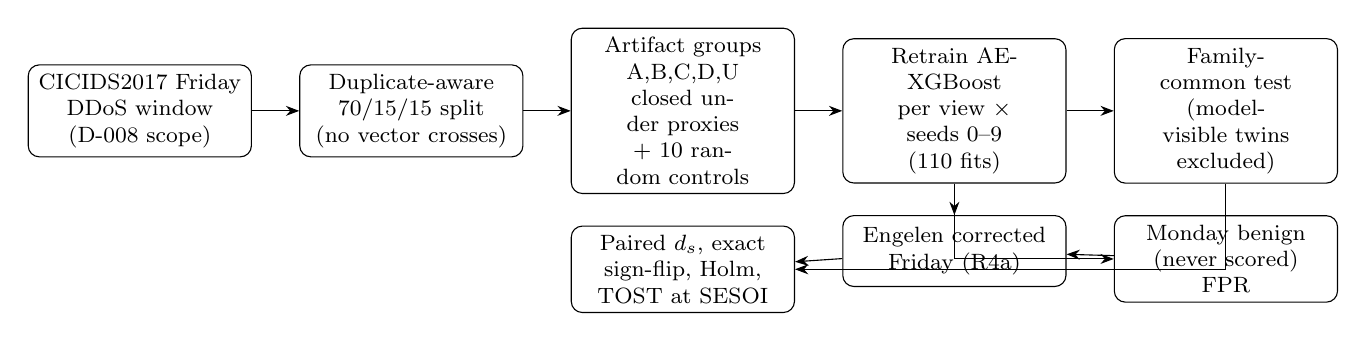
\begin{tikzpicture}[node distance=4mm and 6mm, box/.style={draw, rounded corners, align=center,
  font=\footnotesize, minimum height=9mm, text width=2.6cm}, >=Stealth]
\node[box] (data) {CICIDS2017 Friday\\DDoS window\\(D-008 scope)};
\node[box, right=of data] (split) {Duplicate-aware\\70/15/15 split\\(no vector crosses)};
\node[box, right=of split] (groups) {Artifact groups A,B,C,D,U\\closed under proxies\\+ 10 random controls};
\node[box, right=of groups] (train) {Retrain AE-XGBoost\\per view $\times$ seeds 0--9\\(110 fits)};
\node[box, right=of train] (eval) {Family-common test\\(model-visible twins\\excluded)};
\node[box, below=of eval] (mon) {Monday benign\\(never scored)\\FPR};
\node[box, below=of train] (r4a) {Engelen corrected\\Friday (R4a)};
\node[box, below=of groups] (stats) {Paired $d_s$, exact\\sign-flip, Holm,\\TOST at SESOI};
\draw[->] (data) -- (split); \draw[->] (split) -- (groups); \draw[->] (groups) -- (train);
\draw[->] (train) -- (eval); \draw[->] (train) |- (mon); \draw[->] (train) -- (r4a);
\draw[->] (eval) |- (stats); \draw[->] (mon) -- (r4a); \draw[->] (r4a) -- (stats);
\end{tikzpicture}
\caption{Audit pipeline for the AE-XGBoost main experiment. The DCNN and MES-DNN audits reuse
the leakage controls (Sections~\ref{sec:dcnn}--\ref{sec:mes}).}
\label{fig:pipeline}
\end{figure*}

\subsection{Problem formulation}
Let $\mathcal{D}=\{(\mathbf{x}_i,y_i)\}$ be labelled flows with $y_i\in\{0,1\}$ (1 = attack) and let
$\phi(\mathbf{x})$ denote the \emph{model-visible} input: the float32 vector after preprocessing
and feature selection. A classifier $f_\theta$ trained on a feature subset $S$ is written
$f_{S,\theta}$. For a test population $T$ the error rate is
$\mathrm{ER}(f;T)=|T|^{-1}\sum_{i\in T}\mathbb{1}[\hat y_i\neq y_i]$ with
$\hat y_i=\mathbb{1}[f(\mathbf{x}_i)\geq 0.5]$, and the false-positive rate on benign traffic
$B$ is $\mathrm{FPR}(f;B)=|B|^{-1}\sum_{i\in B}\hat y_i$.

\subsection{Duplicate-aware partitioning and twin exclusion}
Rows are grouped into equivalence classes $[\mathbf{x}]=\{j:\phi(\mathbf{x}_j)=\phi(\mathbf{x})\}$.
The split assigns every class to exactly one of train, validation and test. Because every
ablated view changes $\phi$, a test row may acquire a training twin after columns are removed.
We therefore evaluate every model on the \emph{family-common} population
\begin{equation}
T^\star = \bigcap_{S\in\mathcal{V}} \{\, i\in T : \phi_S(\mathbf{x}_i)\notin\phi_S(X_{\text{train}})\,\},
\end{equation}
where $\mathcal{V}$ is the set of all views (full model, groups and controls).

\subsection{Artifact groups and size-matched controls}
Groups are defined from the literature before training: A (TCP flag-count defects), B (TCP
appendix features), C (duplicated-packet timing features), D (metadata hypotheses such as
destination port) and U (their union). Each group $G$ is closed under the proxy relation measured
on training data (exact equality or $|r|\geq 0.999$), so a removed feature cannot be recovered
through a near-copy. For each $G$ ten random controls $R_{G,1..10}$ of equal size are drawn from
the non-registered, proxy-closed features.

\subsection{Estimand and tests}
For seed $s\in\{0,\dots,9\}$ the effect of removing a set $S$ is
$\Delta_S^{(s)}=\mathrm{ER}(f_{\overline{S},s};T^\star)-\mathrm{ER}(f_{\text{full},s};T^\star)$, and
the control-adjusted paired difference is
\begin{equation}
d_s = \Delta_{G}^{(s)} - \Delta_{R_{G,s}}^{(s)},
\end{equation}
where control draw $s$ is trained with seed $s$. A positive $\bar d$ means removing the
group hurts more than removing random features. Under the sharp null of exchangeability the
exact sign-flip p-value is
\begin{equation}
p=\frac{1}{2^{10}}\sum_{\boldsymbol{\epsilon}\in\{\pm1\}^{10}}
\mathbb{1}\Big[\big|\textstyle\sum_s\epsilon_s d_s\big|\geq\big|\textstyle\sum_s d_s\big|\Big].
\end{equation}
The primary family has ten tests (five groups $\times$ \{error rate, Monday FPR\}), Holm-corrected.
Practical equivalence is declared when the TOST interval lies within the smallest effect size of
interest, $\pm0.001$ (about 33 errors on the test population, and 0.1 percentage points of FPR).

\subsection{Attribution: ARR@K}
For a model's global mean-$|\mathrm{SHAP}|$ ranking, the artifact reliance ratio
$\mathrm{ARR@}K=|\mathrm{top}_K\cap\mathcal{R}|/K$ is the share of the top-$K$ features in the
artifact registry $\mathcal{R}$. It is descriptive only.

\begin{algorithm}[t]
\caption{Feature-reliance audit (one group $G$)}
\label{alg:audit}
\begin{algorithmic}[1]
\Require data $\mathcal{D}$, registry $\mathcal{R}$, group $G$, seeds $s=0..9$
\State split $\mathcal{D}$ by equivalence classes of $\phi$ \Comment{no vector crosses partitions}
\State $G\gets\mathrm{closure}(G)$; draw controls $R_{G,s}$, $|R_{G,s}|=|G|$
\State compute $T^\star$ over all views
\For{$s=0$ to $9$}
  \State train $f_{\text{full},s}$, $f_{\overline{G},s}$, $f_{\overline{R_{G,s}},s}$ with seed $s$
  \State $d_s\gets\Delta^{(s)}_G-\Delta^{(s)}_{R_{G,s}}$ on $T^\star$; same for Monday FPR
\EndFor
\State $p\gets$ exact sign-flip p of $\{d_s\}$; Holm across the family; TOST at SESOI
\State \Return $\bar d$, interval, adjusted $p$, equivalence verdict
\end{algorithmic}
\end{algorithm}

\subsection{Baseline audits}
\label{sec:dcnn}
\textbf{DCNN + self-attention.} The model of Fang et al.~\cite{fang2026}, ported from the
authors' released code, is trained on the official UNSW-NB15 training partition (Normal vs DoS)
with train-only preprocessing and a train-only LightGBM-SHAP selection of 22 features. Each of
five seeds is scored on the official test partition and on the duplicate-filtered test
population (test rows whose model-visible input equals a training row removed).

\label{sec:mes}
\textbf{MES-DNN.} Following Wardana et al.~\cite{wardana2026}, a 39-9-7-5-3-1 DNN is trained per
network and a frozen-base meta-model (10 ReLU units) is trained on held-out meta samples. We use
two networks (NF-UNSW-NB15-v2 and a fixed NF-ToN-IoT-v2 subsample) and compare a random split
with a duplicate-aware split in which each exact input vector occupies one partition.

% ===================================================================== 7. Experimental setup
\section{Experimental Setup}
\subsection{Datasets}
\begin{table}[t]
\centering
\caption{Datasets and populations.}
\label{tab:data}
\begin{tabular}{@{}lrr@{}}
\toprule
Population & Rows & Attack \\
\midrule
CICIDS2017 Fri.\ test, family-common (r1) & 33,038 & 19,233 \\ % results/protocol/milestone3a/eval_population_3a_r1.json
CICIDS2017 Monday benign (twins excluded) & 494,940 & 0 \\ % results/protocol/milestone3b/monday_population_r1.json
Engelen Fri.\ test, family-common (R4a) & 22,049 & 14,168 \\ % results/protocol/r4a/eval_population_r4a_v1.json
UNSW-NB15 train (Normal+DoS) & 68,264 & 12,264 \\ % results/dcnn_fang/selection.json
UNSW-NB15 test, official & 41,089 & 4,089 \\
UNSW-NB15 test, duplicate-filtered & 37,759 & 2,621 \\
NF-UNSW-NB15-v2 & 2,390,275 & 95,053 \\ % configs/datasets.yaml
NF-ToN-IoT-v2 subsample & 2,390,275 & 1,529,289 \\ % results/protocol/mesdnn/ton_subsample_v1.json
\bottomrule
\end{tabular}
\end{table}
CICIDS2017~\cite{sharafaldin2018} is restricted to the Friday afternoon DDoS window (DDoS vs
BENIGN). Engelen's corrected capture~\cite{engelen2021} is aligned to the original clock by a
+5:00 offset; this is an empirically supported assumption validated on the attack onset, not a
confirmed time-zone correction. UNSW-NB15~\cite{moustafa2015} uses the publisher's partitions.
NetFlow-v2 data~\cite{sarhan2022} use the 39 non-identifier features.

\subsection{Implementation and compute}
AE-XGBoost (configs/experiments/ae\_xgb\_d008\_trackB.yaml): AE with one 80-unit hidden layer
around a 40-unit ReLU latent code (68 inputs for the full model), Adam $10^{-3}$, batch 256, at
most 100 epochs with patience 10; XGBoost on the 40 latent codes (lr 0.11, depth 6, at most 2,000
trees with 50-round validation early stopping). Trained on Google Colab (Tesla T4) under a
frozen, fingerprinted environment. DCNN and MES-DNN: PyTorch on a laptop CPU.

\subsection{Metrics}
Error count and rate, MCC, FPR, per-class precision/recall/F1 and ROC-AUC, at a fixed threshold
of 0.5. The positive class is the attack (DoS for UNSW-NB15; Fang et al. use Normal as positive,
so both class-conditional views are reported).

% ===================================================================== 8. Results
\section{Results and Analysis}
\subsection{AE-XGBoost: full model}
Ten full-model seeds made 8, 6, 6, 6, 7, 3, 4, 8, 5 and 5 errors on the 33,038-row
family-common test (mean 5.8; MCC $\approx$ 0.99964). % results/colab results/batch0/SUMMARY.md
\subsection{AE-XGBoost: group ablations (H1) and Monday FPR (H2)}
\pending{Table of $\bar d$, interval, Holm-adjusted p and TOST verdict for groups A--U from
results of batches 1--10 (aggregate\_3b, stats\_3b).}
\subsection{Transfer to the corrected capture (R4a)}
\pending{R4a-i descriptive scores and R4a-ii 70-fit results; observational, not causal.}
\subsection{DCNN + self-attention on UNSW-NB15}
\pending{Five-seed mean and range on official vs duplicate-filtered test, from results/dcnn\_fang/summary.json.}
\subsection{MES-DNN on NetFlow-v2}
\pending{Random vs duplicate-aware ensemble metrics per network, from results/mes\_dnn/summary.json.}
\subsection{Attribution}
\pending{ARR@K for AE-XGBoost (registry v2); DCNN and MES-DNN attribution pilots without ARR
classification (no registry exists for those datasets).}

% ===================================================================== 9. Comparison
\section{Comparison with Base Papers and State-of-the-Art}
Our numbers are not directly comparable with the source papers: the data scope, splits,
populations and polarity differ (Table~\ref{tab:related}). Nezhadsistani et al.\ report F1 0.9993
on CICIDS2017 under 5-fold CV with joint 5G training; Fang et al.\ use a stratified 70/30 split
with Normal as the positive class; Wardana et al.\ use five networks and a random split.
\pending{Side-by-side table: author-reported vs ours, with every protocol difference in a column.}

% ===================================================================== 10. Ablation
\section{Ablation Study}
\pending{Feature-group ablations (main), selector size K = 22 vs the 95\% rule (30 features) for
the DCNN if run, split mode for MES-DNN, and the attention ablation if run.}

% ===================================================================== 11. Discussion
\section{Discussion}
\pending{Interpretation after results; threats to validity: inspected test set (H1 is a
pre-registered estimate, not confirmatory), single capture day, +5:00 alignment assumption,
adaptation differences, sign-flip exactness only under sharp exchangeability, ten seeds.}

% ===================================================================== 12. Conclusion
\section{Conclusion and Future Work}
\pending{Answer to the research question from verified results; future work: other captures,
other attack types, causal attribution methods.}

% ===================================================================== 13. Declarations
\section*{Declarations and Acknowledgements}
\textbf{Data availability.} All datasets are public and were obtained from their official
sources; none is redistributed. \textbf{Code availability.} \pending{repository link or archive}.
\textbf{Funding.} None. \textbf{Competing interests.} None.
\textbf{Use of AI tools.} An AI coding assistant (Anthropic Claude, via Claude Code) helped write
and test the experiment code, extract information from the source papers and draft this
manuscript. The authors specified the research question and approved every protocol decision;
all numbers were produced by the authors' experiments and checked against the result records.
The authors take full responsibility for the content.
\textbf{Acknowledgements.} Experiments used the free tier of Google Colab.

% ===================================================================== 14. References
\bibliographystyle{IEEEtran}
\bibliography{references}

\end{document}
